\documentclass[tikz,border=10pt]{standalone}
\usetikzlibrary{patterns,decorations.pathreplacing}
\usepackage{amsmath,amssymb}
\usepackage{pgfplots}
\pgfplotsset{compat=1.18}
\usepgfplotslibrary{fillbetween}
\begin{document}
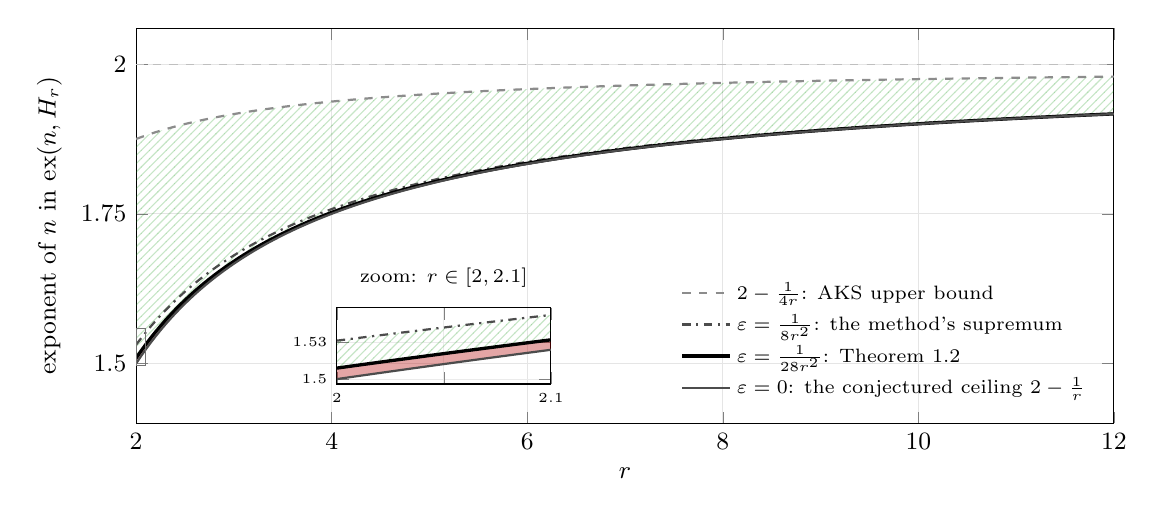
\begin{tikzpicture}
\begin{axis}[name=main,
  width=14cm, height=6.6cm,
  xlabel={$r$}, ylabel={exponent of $n$ in $\mathrm{ex}(n,H_r)$},
  xmin=2, xmax=12, xtick={2,4,6,8,10,12},
  ymin=1.4, ymax=2.06, ytick={1.5,1.75,2},
  yticklabels={$1.5$,$1.75$,$2$},
  grid=major, grid style={black!10},
  every axis label/.append style={font=\small},
  tick label style={font=\small},
  legend style={font=\scriptsize, draw=none, fill=none,
    at={(0.985,0.035)}, anchor=south east},
  legend cell align=left]

\addplot[domain=2:12, samples=100, dashed, black!25, forget plot] {2};

\addplot[name path=aks, domain=2:12, samples=100, thick, black!45, dashed]
  {2 - 1/(4*x)};
\addlegendentry{$2-\frac1{4r}$: AKS upper bound}
\addplot[name path=sup, domain=2:12, samples=200, thick, black!70, dash dot]
  {2 - 1/x + 1/(8*x^2)};
\addlegendentry{$\varepsilon=\frac1{8r^2}$: the method's supremum}
\addplot[name path=ours, domain=2:12, samples=200, very thick]
  {2 - 1/x + 1/(28*x^2)};
\addlegendentry{$\varepsilon=\frac1{28r^2}$: Theorem 1.2}
\addplot[name path=ceil, domain=2:12, samples=200, thick, black!70]
  {2 - 1/x};
\addlegendentry{$\varepsilon=0$: the conjectured ceiling $2-\frac1r$}

\addplot[pattern=north east lines, pattern color=green!55!black,
  opacity=0.22, forget plot] fill between[of=ours and aks];
\addplot[red!70!black, fill opacity=0.35, forget plot]
  fill between[of=ceil and ours];

\draw[black!55, thin] (axis cs:2,1.496) rectangle (axis cs:2.1,1.558);
\end{axis}

% zoom on the widest part of the margin, at small r
\begin{axis}[name=inset, at={(2.55cm,0.5cm)}, anchor=south west,
  width=4.3cm, height=2.55cm,
  xmin=2, xmax=2.1, xtick={2,2.05,2.1}, xticklabels={$2$,,$2.1$},
  ymin=1.496, ymax=1.558, ytick={1.5,1.53}, yticklabels={$1.5$,$1.53$},
  tick label style={font=\tiny}, axis background/.style={fill=white},
  title={\scriptsize zoom: $r\in[2,2.1]$}, title style={yshift=-2pt},
  grid=major, grid style={black!8}]
\addplot[name path=isup, domain=2:2.1, samples=100, thick, black!70,
  dash dot] {2 - 1/x + 1/(8*x^2)};
\addplot[name path=iours, domain=2:2.1, samples=100, very thick]
  {2 - 1/x + 1/(28*x^2)};
\addplot[name path=iceil, domain=2:2.1, samples=100, thick, black!70]
  {2 - 1/x};
\addplot[pattern=north east lines, pattern color=green!55!black,
  opacity=0.22, forget plot] fill between[of=iours and isup];
\addplot[red!70!black, fill opacity=0.35, forget plot]
  fill between[of=iceil and iours];
\end{axis}
\end{tikzpicture}
\end{document}
